\section{Résolution d'un Snake Cube}
L'objectif visant à résoudre un Snake Cube est atteins. Notre application propose divers Snake Cube et les résout en un temps raisonnable (voir Chapitre~\ref{Tests}). En plus de résoudre des Snake Cube classique, c'est à dire dont la forme finale est un cube, notre application peut également résoudre des Snake dont la forme finale est plus complexe. Nous avons par exemple créer un Snake dont la forme finale peut être apparenté à un temple maya (\verb|snake_maya_temple.snake|).

\begin{figure}[h]
 \centering
 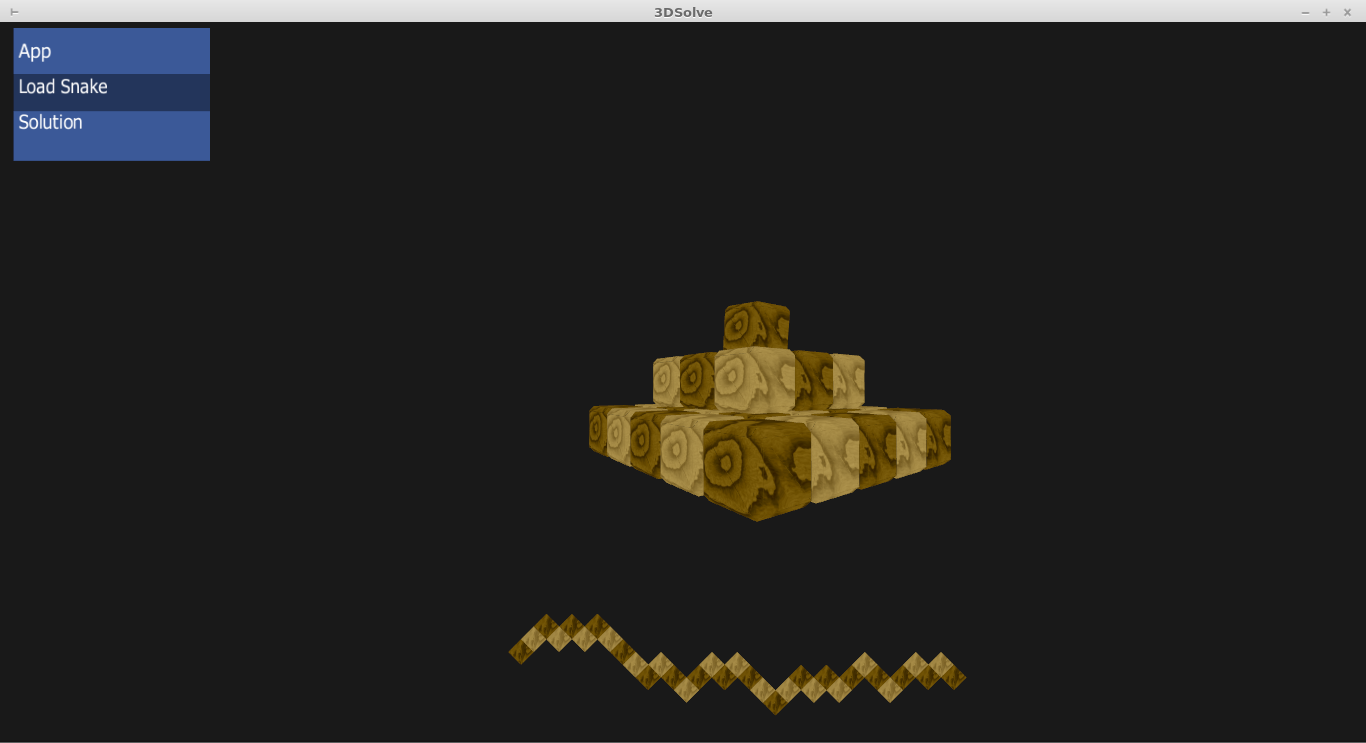
\includegraphics[scale=0.3,keepaspectratio=true]{img/screenShot3.png}
 \caption{``Temple maya'' résolu}
 \label{screenShot3}
\end{figure}

L'interface de rendu 3D propose à l'utilisateur de visualiser, à son rythme, les diverses solutions menant à la résolution du casse-tête sélectionné.

\newpage
\section{Interactivité avec l'utilisateur}
L'objectif d'interactivité avec l'utilisateur, autrement dit la possibilité donné à l'utilisateur de résoudre lui-même le casse-tête, est également atteint. En effet, notre application propose une interface 3D permettant à l'utilisateur de manipuler virtuellement le casse-tête et finalement, un pris d'un effort cérébrale non-négligeable, de le résoudre.

\begin{figure}[h]
 \centering
 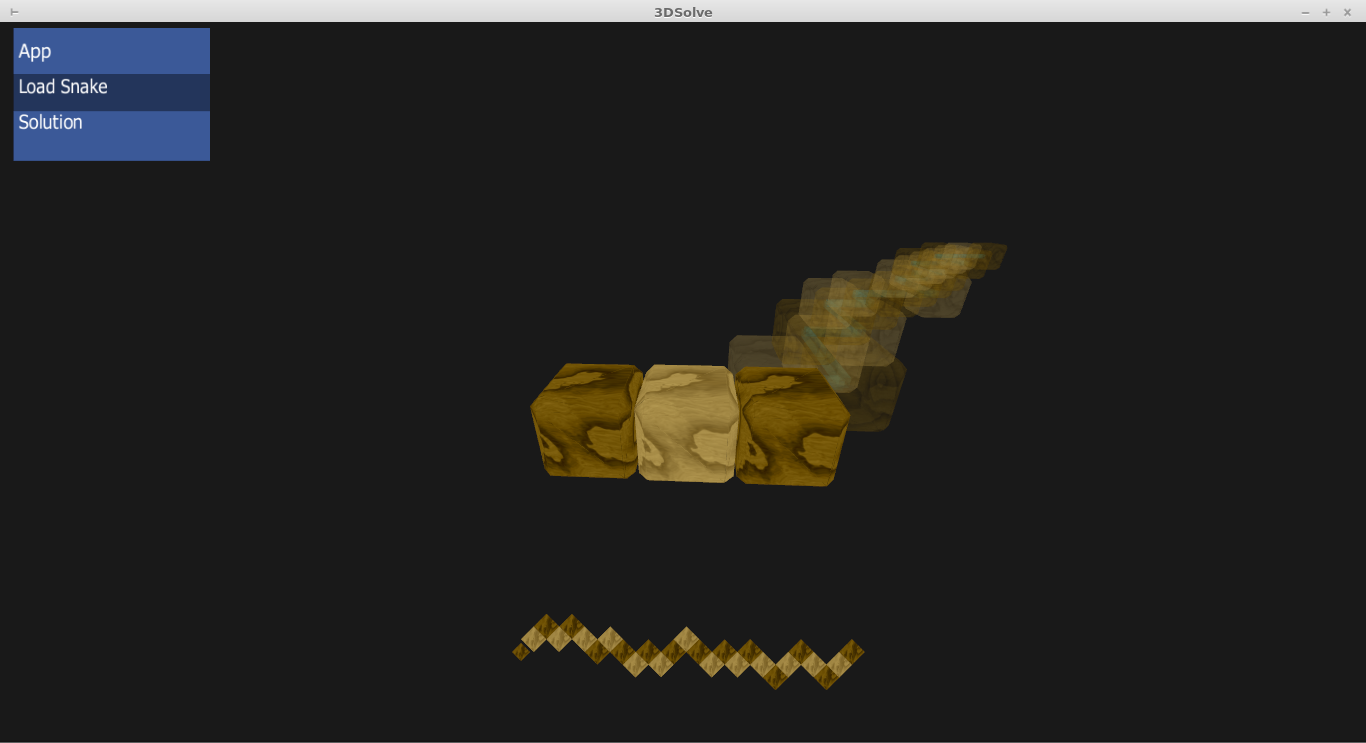
\includegraphics[scale=0.3,keepaspectratio=true]{img/screenShot1.png}
 \caption{Snake Cube déplié en attente de résolution}
 \label{screenShot1}
\end{figure}

\section{Amélioration proposée}
Nous avons eu diverses idées que nous aurions aimé implémenté si nous avions eu plus de temps. Nous les avons regroupées ici sous une seul et même proposition d'amélioration.

L'amélioration consiste en un éditeur de snake. Cet éditeur, sous la forme d'une interface dans le contexte de rendu 3D, permettrait à l'utilisateur de créer ses propres casse-tête.

En premier lieu, l'éditeur pourrait proposer à l'utilisateur de définir un volume en 3D puis de passer ce volume à un algorithme qui effectuerait le travail inverse de l'algorithme de résolution. C'est-à-dire qu'à partir du volume qui lui est donné, il créer un ou plusieurs enchaînement d'unité de snake et créé donc un casse-tête. Le snake ainsi créé pourrait ensuite être sauvegardé dans le format définit au chapitre~\ref{ch6} et être ensuite utilisé comme les autres snake dans la partie interactive de l'application.

Ensuite, on pourrait également imaginer que cet éditeur permette à l'utilisateur de définir non seulement un volume mais également l'enchaînement des unités du snake afin de modéliser un snake réel qui n'est pas proposé par l'application.
